\documentclass[runningheads,a4paper]{llncs}

\usepackage{amssymb}
\setcounter{tocdepth}{3}
\usepackage{graphicx}
\usepackage{subfig}
%\linespread{2}

\usepackage{url}
\usepackage{csquotes}
\newcommand{\keywords}[1]{\par\addvspace\baselineskip
\noindent\keywordname\enspace\ignorespaces#1}

\usepackage{listings}
\usepackage{color}
\usepackage{enumitem}
\usepackage{hyperref}

\definecolor{dkgreen}{rgb}{0,0.6,0}
\definecolor{gray}{rgb}{0.5,0.5,0.5}
\definecolor{mauve}{rgb}{0.58,0,0.82}

\lstset{frame=tb,
  language=C++,
  aboveskip=3mm,
  belowskip=3mm,
  showstringspaces=false,
  columns=flexible,
  basicstyle={\small\ttfamily},
  numbers=left,
  numberstyle=\tiny\color{gray},
  keywordstyle=\color{blue},
  morekeywords={vector},
  commentstyle=\color{dkgreen},
  stringstyle=\color{mauve},
  breaklines=true,
  breakatwhitespace=true,
  tabsize=3
}

\begin{document}

\mainmatter  % start of an individual contribution

% first the title is needed
\title{c3particles: \\ Modeling a Particle System in C++}

% a short form should be given in case it is too long for the running head
\titlerunning{c3particles}

%
\author{Rosalie Kletzander}
%
\authorrunning{c3particles}
% (feature abused for this document to repeat the title also on left hand pages)

\institute{Practical Course "Advanced Software Development with Modern C++"\\Summer Term 2018\\Institute for Computer Science\\
Ludwig-Maximilians-Universit\"at M\"unchen\\
}

\maketitle


\section{Introduction}
Particle systems are used in many different areas: most prominently in the entertainment industry in games and movies and for simulations and visualizations scientific research. No matter the area of application, the basic rules governing these systems are the same: the laws of physics. c3particles (cpp particles) implements a model of a particle system in C++ that separates the physical concepts and laws from the underlying graphics library. This enables a mathematical formulation of the forces influencing the particles.


\section{A Short Recap of Mechanical Physics}

In order to model a particle system that simulates natural phenomena, it is necessary to first understand the basic rules of motion.

Newton's First Law of Motion states:
\begin{quotation}
``Every object in a state of uniform motion tends to remain in that state of motion unless an external force is applied to it." \cite{Newton}
\end{quotation}

This means that an object will not move unless it is accelerated by a force, which brings us to Newton's Second Law of Motion:
\begin{quotation}
``The relationship between an object's mass \emph{m}, its acceleration \emph{a}, and the applied force \emph{F} is $ F = m*a $."  \cite{Newton}
\end{quotation}

With this information it is possible to calculate the acceleration of an object by dividing the applied force by the object's mass. The next step is deriving the velocity and location of the object per time step by integration \cite{strommer}.

The velocity of an object can be calculated by integrating the acceleration over time t. 
\begin{equation}
\overrightarrow{v}(t) = \int \mathrm{(\overrightarrow{a})} \mathrm{d}t = \overrightarrow{a}*t + C_v
\label{eq:vel}
\end{equation}

C is the integration constant, in this case it is equal to the velocity of t-1 for discrete time steps. Integrating the velocity over t yields the location.

\begin{equation}
\overrightarrow{s}(t) = \int \mathrm{(\overrightarrow{v})} \mathrm{d}t = \int (\overrightarrow{a}*t + C_v) \mathrm{d}t = \frac{\overrightarrow{a}*t^2}{2} + C_v + C_s
\label{eq:loc}
\end{equation}

Analogous to $C_v$, $C_s$ is equal to the location at t-1.

With these formulas, it is possible to calculate an object's change in location over time.

A further basic law of physical mechanics is the superposition principle, which states that applying the sum of two forces to an object has the same effect as if they were applied individually. Or, more formally:

\begin{equation}
f(a * x) = a * f(x)
\label{eq:superpos1}
\end{equation}
\begin{equation}
f(x + y) = f(x) + f(y)
\label{eq:superpos2}
\end{equation}

\cite{wiki}

These laws serve as the foundations of the physical model of the particle system. 

\section{Modeling the Particle System}
The basic concepts needed in order to model the particle system are already given by the physics described in the previous section. In fact, a particle system is a fairly simple construct. It contains objects, which behave according to newtonian physics, i.e. "Newtonian Objects". They have a location, velocity, acceleration and mass. As Newton's First Law states, a force needs to be exerted in order for a particle to move. "Force" is therefore the other basic concept.
The concepts "Newtonian Object" (NO) and "Force" are already sufficient for modeling the system, so their expressions must cover all of the basic laws of physics discussed above.

\subsection{Newtonian Object}

\subsubsection{$F = m*a$}
The expression that represents this law is "apply\_force", or "$<<$" and it applies a force to an NO by dividing the force by the NO's mass and adding that to the NO's current acceleration

\subsubsection{Integrating the acceleration}
Using the formulas \ref{eq:vel} and \ref{eq:loc}, the expression "update" calculates an NO's location and velocity from its acceleration

\subsection{Force}

\subsubsection{Force Origins}
Forces are defined by the laws of nature, e.g. gravitational forces. The expression "calc\_force" calculates the force between two NO's according to a given force function

\subsubsection{Superposition Principle}
The expression "accumulate" sums up a set of forces according to the superposition principle.


%\subsection{Time}
%As the particle system is made to be rendered on a screen in (semi) real time, the frame per second count gives discrete time steps that are used for integrating over acceleration. For each frame, one time step is calculated, which simplifies the result of formula~\ref{eq:loc}:
%\begin{equation}
%\frac{\overrightarrow{a}*t^2}{2} + C_v + C_s = \frac{\overrightarrow{a}}{2} +C_v + C_s
%\label{eq:simpleloc}
%\end{equation}

%examples why it is cool: reverse, 

\section{Implementation}

c3particles contains several separate modules (Figure~\ref{fig:sysdia}). The Particle System module contains the physical model and uses input given by the user to select forces. It updates the particles that are then read by the Particle Renderer, which uses the location to calculate the vertices and faces that need to be drawn. It passes the vertex buffers of all the particles to the OpenGL Rendering Pipeline, which processes them accordingly. It then writes the framebuffer to the screen and triggers a new calculation.

\textbf{
\begin{figure}[]
\centering
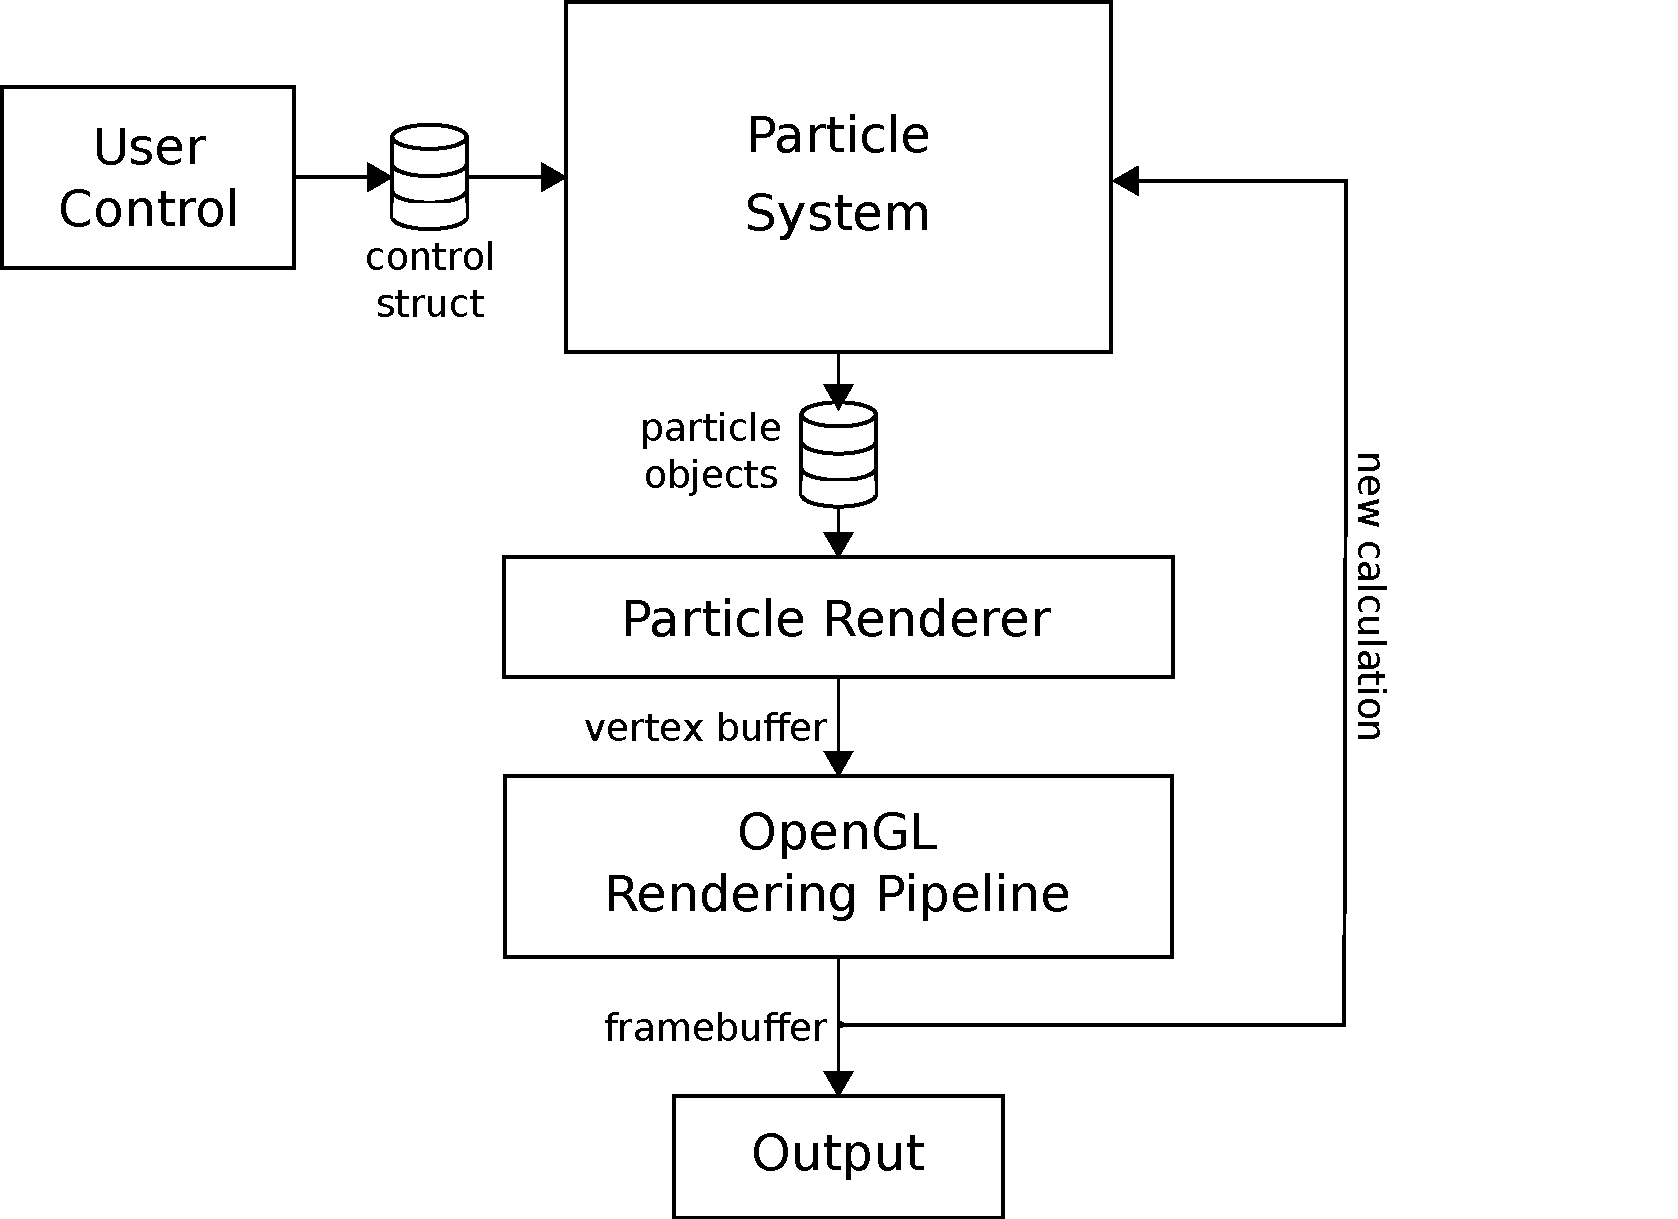
\includegraphics[width=0.8\textwidth]{images/system-diagram-no-shaders.pdf}
\caption{c3particles system diagram}
\label{fig:sysdia}
\end{figure}
}

\subsection{Particle System}
The Particle System module contains the physical model of the particle system and the particle objects (Figure~\ref{fig:sysdiadetail})

The physical model includes algorithms for calculating the forces on the particles, and the particles themselves. For each frame, the old values of the particles are read and used to update to the new values. This is where the previously defined expressions are relevant.

\textbf{
\begin{figure}[]
\centering
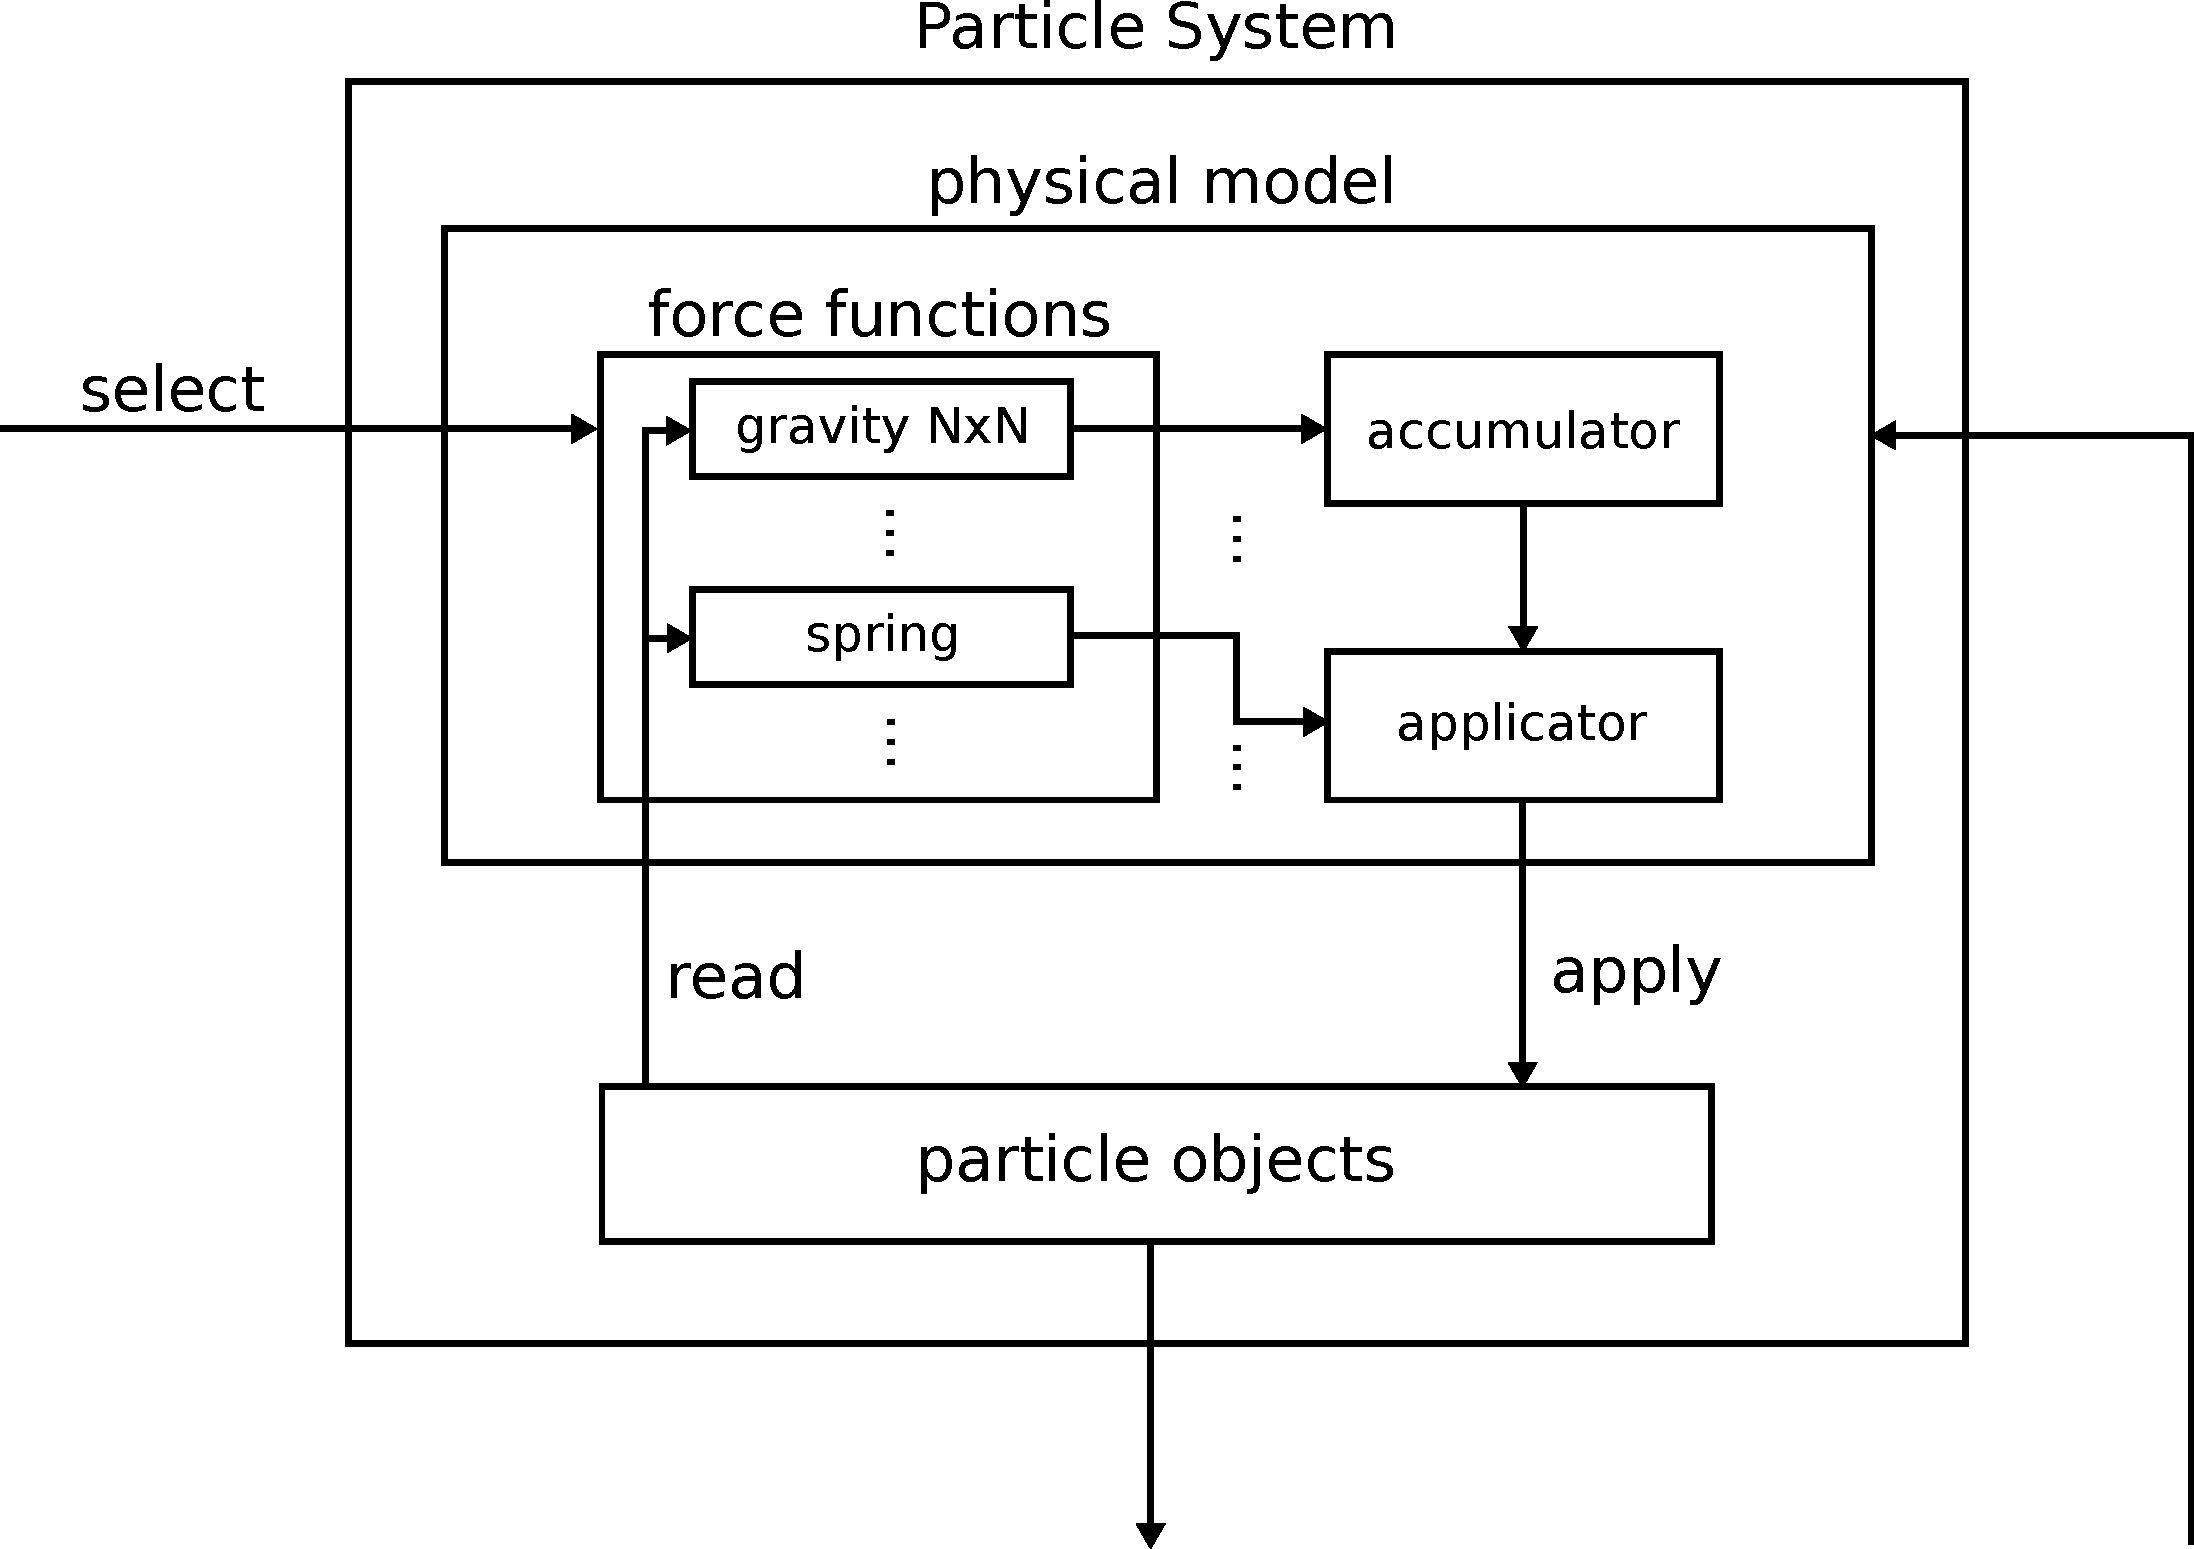
\includegraphics[width=0.8\textwidth]{images/particle-system-detail.pdf}
\caption{detailed diagram of the particle system}
\label{fig:sysdiadetail}
\end{figure}
}

\subsubsection{Algorithms}

First, selected force functions are computed for each particle in the system. These functions are all based on calc\_force~\ref{fig:calcforce} which calculates the force between two particles based on a lambda function. 

\begin{lstlisting}[caption=calc\_force function]
// calculates a force between two particles using the function ff
// when given the same particle twice, it returns the additive identity
Force calc_force(
    const Particle &p1,
    const Particle &p2,
    std::function<Force(const Particle &p1, const Particle &p2)> ff)
{
  if (&p1 == &p2)
    { return Force(0, 0, 0); }
  return ff(p1, p2);
}                                    
\end{lstlisting}
 \label{fig:calcforce}

This enables very straightforward definition of any force between two particles. It can be used to describe forces on the fly, or to create pre-defined force functions, such as gravitational force (Listing~\ref{fig:gravity}).

\begin{lstlisting}[caption=gravity function]
// uses calc_force to calculate gravitational force between two particles
Force gravity(const Particle &p1, const Particle &p2, float g_constant)
{
  Force result = calc_force(p1, p2, 
						[p1, p2](const Particle &, const Particle &) {
	glm::vec3 direction = p2.location - p1.location;
	float gforce = (p1.mass * p2.mass) / pow(glm::length(direction), 2);
	glm::normalize(direction);

	return g_constant * (gforce * direction);
  });
}               
\end{lstlisting}
 \label{fig:gravity}


For the calculation of the forces it is helpful to split them logically into "inter-particle forces" and "external forces". The former refers to the forces that exist between all pairs of particles (e.g. gravitational forces) and the latter refers to forces that are applied to each particle independently of all others (e.g. wind). This is the reason for the differentiation between forces that are applied directly (e.g. "spring" in Figure~\ref{fig:sysdiadetail}) and forces that are accumulated first (e.g. "gravity in Figure~\ref{fig:sysdiadetail}). Listing~\ref{fig:main} shows an example for the application of different forces on the particles of a particle system.

\begin{lstlisting}[caption=example of how forces are calculated and applied]
//iterate over all particles in the particle system
std::for_each(ps.begin(), ps.end(), [&ps](c3p::Particle& p)
{

  	//gravitational forces between particles
	p << c3p::accumulate(p,
						 ps.particles(),
						 {ps.g_constant()},
    					 c3p::gravity);
    					 
	// spring force from virtual particle at (0,0,0) to each particle
	p << spring(p, Particle(0,0,0), {spring_constant, spring_length);

	// simple user-defined attraction force pulling towards (0,0,0)
	p << calc_force(p, Particle(), [p](const Particle &, const Particle &)
	{
    	glm::vec3 direction = glm::normalize(glm::vec3(0,0,0) - p.location());
		return direction * 0.1;
    });
}          
   
\end{lstlisting}
 \label{fig:main}

\emph{c3p::accumulate} (Listing~\ref{fig:main}, line 6) calculates the forces between each pair of particles (i.e. inter-particle forces) and reduces them. The result is a force that can then be applied directly.

The next step is updating all the particles with the update function (Listing~\ref{fig:update}). The calculation for the current time step is then finished and control is passed to the Particle Renderer.

\begin{lstlisting}[caption=update function]
void update(Particle &p)
{
	//v(t) = a*t + v(t-1)                                                            
	p.velocity = p.acceleration * 1.0f + p.velocity; //deltaT = 1.0                                  
                                                                                           
	//s(t) = (a*t^2)/2 + v(t) + s(t-1)                                               
	p.location = (p.acceleration * 1.0f) / 2.0f + p.velocity + p.location;
                                       	
	//acceleration is not accumulative, but recalculated at each time step          
	p.acceleration = {0, 0, 0};
}                                                            
\end{lstlisting}
\label{fig:update}

\subsection{User Control Window}
The user controls are implemented with GTK+\cite{gtk}. The control window runs in a different thread that fills a C struct with the values set by the user. These values are then read by the system in order to calculate the desired forces.

\subsection{Particle Renderer}
The particle renderer iterates over the particles in the particle system and fills the vertex buffers for each one. How the vertex buffers are filled depends on the function called. At the moment, it is possible to render the particles as pixels with no depth perception and uniform size (\emph{c3p::ParticleRenderer::renderPoints}
or as cubes (\emph{c3p::ParticleRenderer::renderCubes}). The size of the cubes is proportional to the mass of the particle. The vertex buffers are then passed to the OpenGL Rendering Pipeline.

%\subsection{Shaders}

\subsection{Graphics Engine}
The graphics engine is only secondary for this project. OpenGL\cite{opengl} was chosen because of its prominence, however, with an appropriate particle renderer, any one could be used.

\section{Complexity and Possible Optimizations}
The implementation of a particle system has a few areas that inherently have a high time complexity. For example, the complexity of a naive implementation of inter-particle forces is $O(2n^2)$, where every force is calculated twice.

Furthermore, applying a force, updating, and rendering each particle requires $O(3n)$. For systems with a large number of particles, this quickly exceeds the capacities of regular CPU hardware. In order to mitigate this load, there are several possible approaches.

The first and easiest solution would be to parallelize the iterations over the particles. Since applying forces to particles does not change the location and velocity (which would need to be read by other threads), parallelization is no problem at all. The same applies for the update loop.

These functions are also well-suited to be offloaded to the GPU.

The inter-particle NxN forces provide somewhat more of a challenge. A possible solution could be to construct a partitioned semi-symmetric force matrix (the lower half is the inverse of the upper half) and fill two fields after one calculation. Binary space partitioning could also be useful for forces that have a strong distance decay (such as gravity).


\section{Significance of the c3particles Programming Abstraction}

The programming abstraction offered by c3particles allows for a very formal definition of physical forces to be applied to the system. This, along with the clean separation from the underlying rendering pipeline makes implementing new forces very uncomplicated and elegant. 



\bibliography{literature}
\bibliographystyle{plain}

\end{document}
